В рамках секции будут описаны методы, применяемые в генеративном моделировании
для решения задачи генерации задач.


\begin{figure}[h]
    \centering
    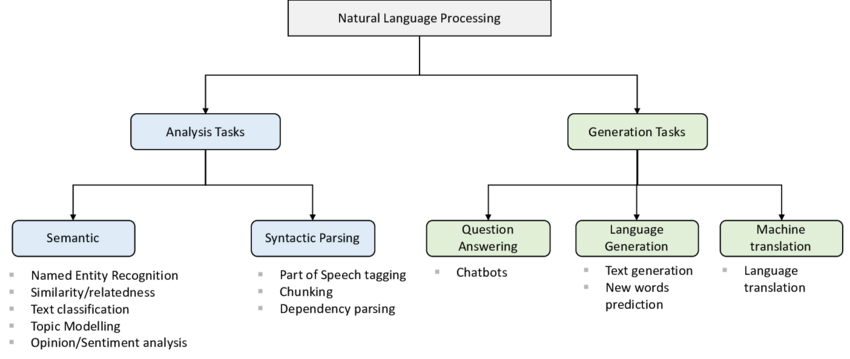
\includegraphics[width=0.5\textwidth]{assets/llm/taxonomy.png}
    \caption{Таксономия современных подходов обработки естественного языка}
    \label{llm_taxonomy}
\end{figure}




\section{Использование нейросетевых подходов}

В рамках раздела будет последовательно изложена хронология подходов
для построения генеративных моделей языка.

 модели строились на n-граммах \cite{heafield-2011-kenlm}
 


В последствии подходы развивились примением реккурентных нейронных сетей LSTM \cite{HochSchm97} и GRU



С эффективным примением архитектуры нейронной сети Attention \cite{NIPS2017_3f5ee243}, позволяющей эффективно обучать нейронные сети на графических ускорителях. 




\section{Обработка естественного языка}

\subsection{Методы обработки естественного языка}

Анализ естественного языка это межпредметная дисциплина.
Компьютерная лингвистика

Практически востребованной оказалась дистрибутивная гипотеза \cite{Schutze},
легшая в основу алгоритма \cite{NIPS2013_9aa42b31}


**Лемматизация** - процесс приведения языка к нормальной форме.

**


\section{Обработка изображений}

\subsection{Методы обработки естественного языка}

Анализ естественного языка это межпредметная дисциплина.
Компьютерная лингвистика

Практически востребованной оказалась дистрибутивная гипотеза \cite{Schutze},
легшая в основу алгоритма \cite{NIPS2013_9aa42b31}


**Лемматизация** - процесс приведения языка к нормальной форме.

**


Наибольшей успех в обработке естественного языка связан с
введением 

Авторегрессионая модель

